\documentclass[aspectratio=169, usenames, dvipsnames]{beamer}

\usepackage{xcolor}
\usepackage[normalem]{ulem} % for strikethrough text

% set up minted
\usepackage{minted}
\setminted{autogobble=true, linenos=false, fontsize=\footnotesize}
\usemintedstyle{friendly}

\definecolor{rustcolor}{rgb}{0.95,0.95,0.95}

% LAST import: menukeys
% \usepackage{menukeys}
% \renewmenumacro{\menu}[>]{roundedmenus}

% for semi transparent text
\newcommand{\semitransp}[2][35]{\textcolor{fg!#1}{#2}}

% setup for footnotes...
\addtobeamertemplate{footnote}{\vspace{-8pt}\advance\hsize-0.5cm}{\vspace{8pt}}
\makeatletter
\renewcommand*{\footnoterule}{\kern -3pt \hrule \@width 2in \kern 10.6pt}
\setbeamerfont{footnote}{size=\tiny}

\title{Ohua as STM Alternative for Shared State Applications}
\subtitle{Master Defense}
\date{25th August 2020}
\author{Felix Wittwer}

\usetheme{ccc}

\begin{document}

\begin{frame}
\titlepage
\end{frame}

\begin{frame}{Shared State Application: Labyrinth Benchmark}
  \begin{columns}
    \begin{column}{0.5\textwidth}
      \textbf{Given:} 3D maze, pairs of points\\[\baselineskip]

      \uncover<2->{\textbf{Goal:} Map a path between each pair of points\\[\baselineskip]}

      \uncover<3->{\textbf{Implementation:}}
      \begin{itemize}
      \item<3-> parallel search for new paths
      \item<4-> merge paths into the maze\\\uncover<5->{$\rightarrow$ retry if path crosses other paths}
      \end{itemize}
    \end{column}
    \begin{column}{0.5\textwidth}
      \begin{center}
        \includegraphics<1-2>[width=.9\textwidth]{img/1-maze_points}%
        \includegraphics<3>[width=.9\textwidth]{img/2-maze_paths}%
        \includegraphics<4>[width=.9\textwidth]{img/4-maze_update2}%
        \includegraphics<5->[width=.9\textwidth]{img/5-maze_update3}%
      \end{center}
    \end{column}
  \end{columns}
\end{frame}


\begin{frame}{Shared State Application: Labyrinth Benchmark}
  \begin{columns}
    \begin{column}{0.5\textwidth}
        \begin{block}{Irregular Applications}
            centered around the manipulation of pointer-based data structures
        \end{block}
        
        \hfill

        \begin{itemize}
            \item<2-> structure makes identification of safe parallel accesses hard
            \item<3-> compiler analyses struggle to uncover meaningful parallelism
        \end{itemize}
    \end{column}
    \begin{column}{0.5\textwidth}
      \begin{center}
        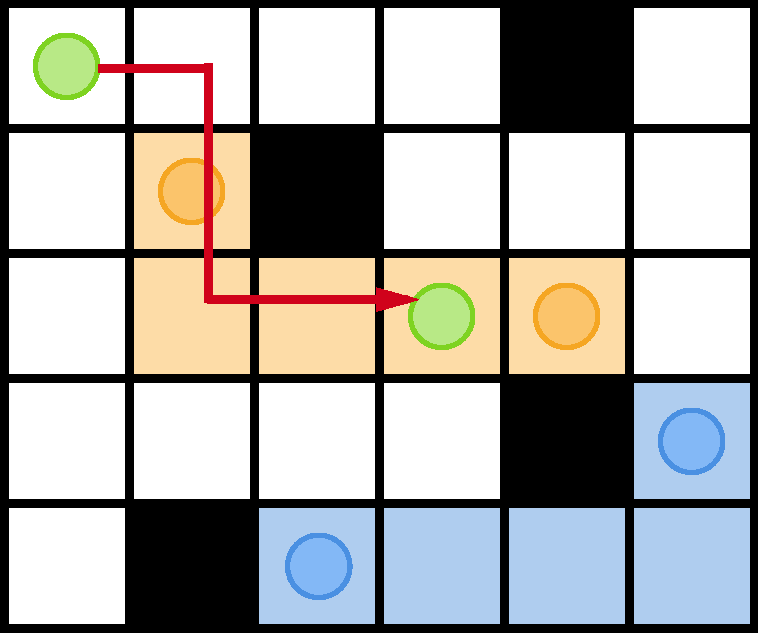
\includegraphics[width=.9\textwidth]{img/5-maze_update3}%
      \end{center}
    \end{column}
  \end{columns}
\end{frame}

\begin{frame}{Shared State Application: Labyrinth Benchmark}
  \begin{columns}
    \begin{column}{0.5\textwidth}
        \begin{block}{Amorphous Data Parallelism}
            behaviour observed in some irregular applications
        \end{block}

        \hfill

        \begin{itemize}
            % \item behaviour observed in some irregular applications\\ \ 
            \item<2-> processing one element may generate new work items or remove others
            \item<4-> some items cannot be processed in parallel due to conflicts
        \end{itemize}
    \end{column}
    \begin{column}{0.5\textwidth}
      \begin{center}
        \includegraphics<1-2>[width=.9\textwidth]{img/5-maze_update3}%
        \includegraphics<3->[width=.9\textwidth]{img/6-maze_update-noconflict}%
      \end{center}
    \end{column}
  \end{columns}
\end{frame}

\begin{frame}{Shared State Applications: Implementation}
    % TODO: Give that slide some love?
    \textbf{Problem:}\\
    \begin{itemize}
        \item Compiler Analyses cannot uncover meaningful parallelism
        \item<2-> Locking is too defensive
    \end{itemize}

    \vspace{1.5em}

    \uncover<3->{\textbf{Solution:} Optimistic Parallelism}
\end{frame}

\begin{frame}[t]{Optimistic Parallelism: Software Transactional Memory\footnotemark[1]}
    \centering%
    \includegraphics<1-2>[width=.8\textwidth,keepaspectratio]{img/background-stm1}%
    \includegraphics<3>[width=.8\textwidth,keepaspectratio]{img/background-stm2}%
    \includegraphics<4>[width=.8\textwidth,keepaspectratio]{img/background-stm3}%
    \includegraphics<5>[width=.8\textwidth,keepaspectratio]{img/background-stm4}%
    \includegraphics<6->[width=.8\textwidth,keepaspectratio]{img/background-stm5}%
    \flushleft

    \begin{itemize}
        \only<1-7>{
            \item uses \emph{transactions} to guard access to shared data
            \begin{itemize}
                \item<2-> work similar to database transactions
                \item<7-> ensure atomicity, consistency and isolation
                % \item<4-> all changes within transaction take effect at once
            \end{itemize}
        }
        \only<8->{
            \item allows shared data access without blocking
            \item<9-> \textbf{optimistic:} assumes only few conflicts will happen
        }
    \end{itemize}
    \footnotetext[1]{Shavit, et al. "Software transactional memory." Distributed Computing 10.2 (1997): 99-116.}
\end{frame}

\begin{frame}{Ohua\footnotemark[2]}
  \begin{columns}
    \begin{column}{0.7\textwidth}
      Framework for implicit parallel programming:\\[.55\baselineskip]
      \begin{itemize}
        \item<2-> Derives dataflow graph from algorithm file
        \item<3-> Runs optimizations on graph to exploit parallelism at compile time
        \item<4-> Generates native runtime code
      \end{itemize}
      % TODO: Zusätzlichen Punkt, der Ohua besser verkauft für dieses Problem.

      \vspace{1.5em}

      \uncover<5->{\textbf{Is Ohua a possible alternative to STM?}}
    \end{column}
    \begin{column}{0.25\textwidth}
      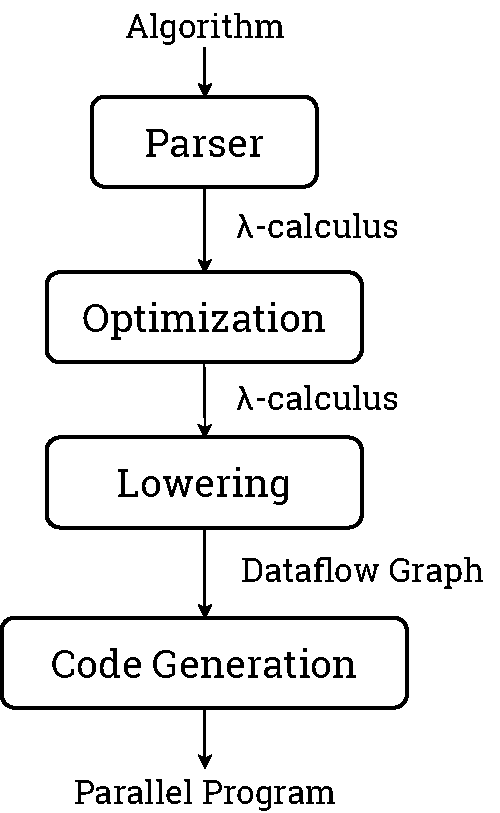
\includegraphics[width=\textwidth,height=\textheight,keepaspectratio]{img/ohua}
    \end{column}
  \end{columns}

  \footnotetext[2]{Ertel et al. "Towards Implicit Parallel Programming for Systems." dissertation, 2019.}
\end{frame}

\begin{frame}{Compiler Transformations}
    % TODO
\end{frame}

\begin{frame}{Performance Comparison}
    \begin{itemize}
        \item measured speedups for STM and Ohua
            \begin{itemize}
                \item<2-> 4 representative benchmarks from STAMP\footnote[3]{Minh, Chi Cao, et al. "STAMP: Stanford transactional applications for multi-processing." 2008 IEEE International Symposium on Workload Characterization. IEEE, 2008.} suite
                \item<3-> 3 different inputs\\ \ 
            \end{itemize}
        \item<4-> Result verification
            \begin{itemize}
                \item<4-> Compare STAMP (C) results with our STM performance (Rust)
            \end{itemize}
        \end{itemize}
\end{frame}

\begin{frame}{Results: Labyrinth}
    \
\end{frame}

\begin{frame}
  \centering
  \huge
  \alert{\textbf{Thank you for your attention.}}
\end{frame}

% -----------------------------------------------------------------------------------------------------------
% ---------------------------------------------- BACKUP Slides ----------------------------------------------
% -----------------------------------------------------------------------------------------------------------

\begin{frame}
  \centering
  \huge
  \alert{\textbf{Backup}}
\end{frame}


\end{document}
